\documentclass[11pt,a4paper]{article}
\usepackage[T1]{fontenc}
\usepackage[utf8]{inputenc}
\usepackage{lmodern,graphicx,booktabs,tabularx,microtype}
\usepackage[margin=25mm]{geometry}
\usepackage[hidelinks]{hyperref}
\hypersetup{pdftitle={Selected Perception Methods},pdfauthor={Ege Gursoy}}
\setlength{\emergencystretch}{2em}
\title{Selected Perception Methods}
\author{Ege Gursoy}
\date{30 October 2026}
\begin{document}
\maketitle
The \path{perception_challenge_best} branch retains the selected stereo hold
estimator, configured robot estimator and persistent RGB robot/cup tracker.
It contains one trained checkpoint, one example per challenge, isolated setup
and camera calibration. Alternatives and historical experiments remain on
\path{perception_challenge_full}. The command reference is
\path{docs/perception/README.md}.

\section{Retained methods}
\textbf{Stereo holds.} Color proposals initialize dual-view exact CAD fitting.
A verified public-generator search can recover an untouched native layout;
failed verification retains the independent CAD estimate. Input is a stereo
PNG and declared rig calibration. Output is \texttt{holds.json}: CAD backplate
anchors in metres, intrinsic XYZ Euler radians, hold type and color.
Exact recovery assumes ten Microban holds, zero to three volumes and the
released generator geometry/appearance. It does not apply to camera photographs.

\textbf{Saved robot frames.} A 20-point Microban network initializes the known
joint configuration. M3T tracks the configured links; protected CAD refinement
and a trimmed boundary fallback estimate the trunk transform. The selected
\texttt{max} profile requires two RGB images, calibrated intrinsics, synchronized
timestamps and all 19 measured joints. It does not reconstruct unknown joints.

\textbf{Continuous perception.} The \texttt{fast} profile retains persistent M3T,
a dense RGB cup map and conditional socket correction. Candidate sockets must
have image support and satisfy geometry gates. Socket proximity does not confirm
seating or loading. Cup geometry and lattice priors require physical measurement.

\begin{figure}[htbp]\centering
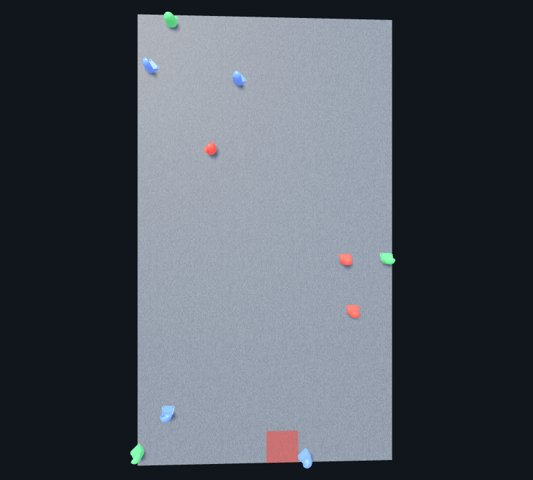
\includegraphics[width=.48\linewidth]{figures/holds.jpg}\hfill
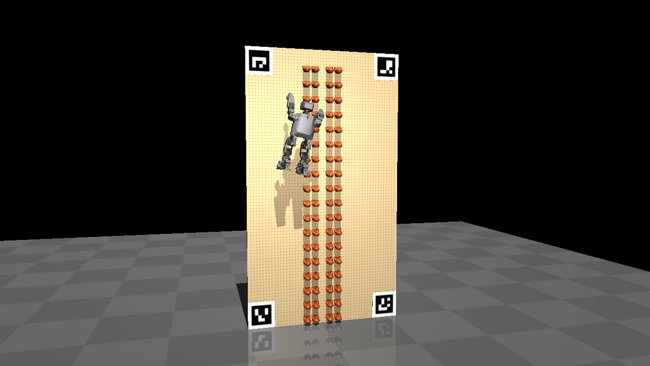
\includegraphics[width=.48\linewidth]{figures/robot.jpg}
\caption{The included stereo hold scene (left view) and configured robot scene
(first camera). Inference uses both views. Saved examples are regression cases.}
\end{figure}

\section{Install and reproduce}
Use Linux x86-64, Python 3.12, Git/Git-LFS, C++ tools, EGL/OpenGL and CUDA 12.8.
The tested GPU is RTX 5000 Ada, compute capability 8.9; change
\texttt{--cuda-arch} during setup for another supported card.
\begin{verbatim}
git submodule update --init
python3.12 scripts/perception/setup.py --robot --cuda
source .venv-perception/bin/activate
python scripts/perception/run.py doctor --robot
python scripts/perception/run.py reproduce --out outputs/holds
python scripts/perception/run.py replay \
  --dataset data/perception/robot --out outputs/robot
python scripts/perception/verify_replays.py \
  --dataset data/perception/robot --predictions outputs/robot \
  --out outputs/robot/verification.json
\end{verbatim}
Setup creates a private environment and cache. Torch/CUDA/native dependencies
still require several GB. GPU jobs wait for spare capacity and poll every
30 minutes while externally busy. The runtime does not stop other jobs.

\section{Cameras and measurements}
\texttt{capture --list} enumerates devices. Select two serials, capture RGB pairs,
then run \texttt{calibrate} on varied printed-board poses. The guide gives the
complete commands. Only color streams are enabled. Intrinsic calibration fits
SDK-rectified frames and is bound to serial order, resolution and source
intrinsics. Wall pose is estimated separately from markers or board boundaries.

Supply a measured encoder JSONL log with \texttt{clock: host\_monotonic},
\texttt{timestamp\_s} and all 19 \texttt{joints\_rad}. Map acquisition times into
the camera laptop's clock; an independent Pi clock or receipt time is insufficient.
\begin{verbatim}
python scripts/perception/run.py live \
  --serial LEFT_SERIAL --serial RIGHT_SERIAL \
  --telemetry-log outputs/encoders.jsonl \
  --camera-calibration outputs/calibration/calibration.json \
  --out outputs/live
\end{verbatim}
Live defaults to combined robot/cup tracking. Use \texttt{--task robot} for root
pose alone. Consumers read \texttt{latest.json} and require \texttt{valid} and
\texttt{fresh}. Poses older than the default 0.25 s limit are suppressed. Inspect
map timestamps and refresh errors separately; reacquisition may take seconds.

The private model reproduces the original simulator. Team main uses the cut-foot
fork. Physical fitting must use the measured geometry through
\texttt{RCR\_MICROBAN\_MODEL}. The guide explains this override and team frame
conversion. A complete team wall model still needs verified start contacts.

\section{Checks and scope}
After removing alternatives, the selected code reproduced all 50 source hold
records on the five saved stereo cases from the full branch. All five robot
cases passed the local root thresholds (5 mm and 5 degrees) and the 5 mm bound
for every endpoint. Combined replay produced a valid robot pose and 72 mapped
cup candidates on the retained example, with no refresh error. Candidate count
is not an independently scored map-accuracy result.

The repository carries only one case per challenge; the compact
\path{verification.json} records the broader saved-case check. References are
opened after inference. These are regression checks, not new blind benchmarks.
Calibration and timing paths have software tests. No physical cameras were
attached, so USB reliability, exposure synchronization, physical accuracy and
a camera-driven climb remain unvalidated. The legacy images-only team functions
remain stubs; use the explicit packet API to supply calibration and telemetry.
\end{document}
